\chapter{Este es el primer capítulo}


\begin{equation}
	\dot {\hat x} = A \hat x + B u + L \left( y - C \hat x \right)  
\end{equation}

 
\begin{figure}
	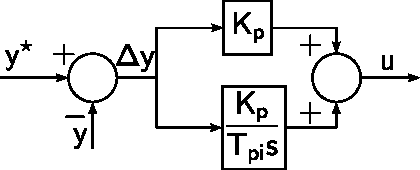
\includegraphics[width=\textwidth]{model/pdf/pi.pdf} 
	\caption{Control proporcional integral}
	\label{ctrl_pi}
\end{figure}
 
 
 \cite{Rodriguez2007}
 
 

